\section{Evaluation}
\label{sec:eval}
We evaluate our ASR system by comparing it with the official
baseline system using GMM (called Baseline) along with several
high ranking algorithms (namely GSR, RNH and OE) downloaded from IEEE AASP
Scene Classification task website\cite{6701819}
on classification of up to 10 scenes.
In addition, we show the most popular sound events detected by our system
for each of these scenes.


\subsection{Experiment Setup}
%In the experiment, we use the same testing data as our previous work\cite{LML}. We download audio clips from SoundJax\footnote{http://soundjax.com/}, FindSounds\footnote{http://www.findsounds.com/}, FreeSound\footnote{http://www.freesound.org} and YouTube\footnote{http://www.youtube.com/}, including sounds of events and sounds of scenes.
Our dataset consists of audio samples of 10 scenes:
{\bf bar}, {\bf beach}, {\bf cafeteria}, {\bf church},
{\bf concert}, {\bf office}, {\bf park}, {\bf street},
{\bf toilet} and {\bf train}.
There are 10 training clips for methods from AASP, no training clips
for our method,
and 10 testing clips for each scene.\footnote{These
clips are obtained by querying the scene words on FreeSound.org and
are available at \url{http://202.120.38.146/~kzhu/audio/}.}
The duration of every
training clip ranges from a few seconds to a few minutes, while all the
testing clips are truncated to 20 seconds long.
All clips are converted to WAVE form with a single channel,
16 bits per sample point, 384kbps bit-rate.
We did not use the IEEE AASP audio data because their clips generally
do not contain detectable events even to the human ear. Instead they
carry global features that are good for traditional ASR modeling.
Moreover, the training and test data appear to be similar to each other,
giving extra advantage to the AASP methods.

We set the frame size to 512 sample points (20ms) with 50\% overlap
to extract audio features.
The MFCC feature are extracted using open source code written by Klautau
in 2001. The implementation is based on \cite{1163420, 237532,397093,
Cardin:1993:ICM:1946943.1947011}. We combine ZCR, 12-dimensional MFCC
and its 1st- and 2nd-order differentials (37 dimensions in total)
to train our GMM models. The number of mixtures in GMM is set to 32.

All experiments are conducted on an Intel Core i7 3.4GHz
desktop computer with 32GB memory, running Windows Server 2012, and all programs
are single-threaded.

\subsection{Event Detection}
Our audible event vocabulary contains 2326 terms.
Total number of contexts extracted from the script corpus
for the 10 scenes is 4953.
%while the total number of audible events detected is 184.
Because not all these events are significant,
to simplify training, we only keep those events which occur
sufficient number of times (0.01\% out of all event terms)
in at least one of the 10 scenes in our text corpus.
As a result, 184 acceptable events were found in these 10 scenes
in the corpus, and these are used to build the even-scene distribution.
%\fig{audible} shows these event terms.

\tabl{te} gives 5 most probable
events detected for each of the scenes. Most of the scenes successfully
have their important events detected in the test samples. However,
some false positive events present, such as ``bark'' which exists in many
scenes. The reason is ``bark'' is a very popular keyword on sound search
engines which return many diverse, noisy audio samples. Consequently,
the model for ``bark'' is relatively coarse and thus can be erroneously
detected almost everywhere. ``Station'' is also detected incorrectly
at several places. This is because ``station'' actually is more of a scene
than a single event, since it is represented by a global ambiance with
noises, vague human speech and perhaps music in the background. Such global
features are present in public areas. ``Urine'' was not detected in the
``toilet'' scene because our samples don't have it.
%We then go on to build the event-scene distribution using these
%events. In total, 15735 audio clips are used to train the audible events
%for 10 scenes.
%
%\begin{figure}[th]
%\centering
%\fbox{\parbox{\columnwidth}{
%\small
%cracker
%teen
%dispenser
%bark
%bell
%{\em commercial}
%dish
%tray
%rod
%teacher
%{\em garbage}
%{\em backpack}
%soup
%egg
%country
%buck
%cup
%club
%chain
%chaos
%{\em video}
%table
%coffee
%tile
%hallway
%student
%steam
%fountain
%fork
%explosion
%angel
%{\em corn}
%chant
%dial
%computer
%kid
%wing
%piano
%file
%stick
%shower
%fist
%trance
%rock
%war
%counter
%son
%family
%drink
%water
%hall
%foil
%tub
%bathroom
%sink
%bathtub
%bath
%{\em medicine}
%{\em barn}
%{\em pearl}
%{\em towel}
%{\em mirror}
%cabinet
%spoon
%bedroom
%cotton
%pill
%hit
%curtain
%scissors
%tank
%square
%can
%drawer
%blast
%rack
%speaker
%tv
%television
%traffic
%bus
%{\em navy}
%vehicle
%coast
%gate
%rifle
%path
%sidewalk
%{\em blanket}
%{\em potato}
%pub
%playground
%match
%microphone
%jam
%{\em ghost}
%speech
%show
%engine
%{\em mud}
%grocery
%taxi
%christmas
%{\em sun}
%telephone
%town
%stadium
%song
%thumb
%applause
%{\em tower}
%ocean
%beer
%station
%yard
%cab
%river
%boat
%sea
%soldier
%shop
%store
%{\em pumpkin}
%hardware
%{\em pizza}
%register
%bin
%factory
%rip
%belt
%gorilla
%desert
%stone
%{\em bridge}
%ship
%passenger
%present
%bike
%pencil
%van
%jungle
%roof
%santa
%king
%{\em bench}
%{\em furniture}
%rope
%bush
%chopper
%trailer
%carriage
%village
%sand
%jeep
%pavement
%ticket
%pigeon
%subway
%grill
%dolphin
%devil
%shell
%satellite
%grass
%{\em craft}
%coach
%viola
%goat
%tunnel
%cliff
%zoo
%ammunition
%choir
%shore
%keyboard
%railroad
%cabin
%communication
%espresso
%cello
%dagger
%surf
%peanut
%teapot
%}}
%\caption{184 Audible Events Extracted for 10 Test Scenes}
%\label{fig:audible}
%\end{figure}

\begin{table}[th]
\centering
\small
\caption{Top 5 Detected Events per Scene}
\label{tab:te}
\begin{tabular}{l|ccccc}
\toprule
{\bf Scene} & \multicolumn{5}{c}{{\bf Events}}\\
\hline
street & traffic & engine & station & bark & subway\\ \hline
office & bark & dish & bike & backpack & bathroom\\ \hline
beach & sea & water & sand & river & shore\\ \hline
concert & applause & bark & tv & tunnel & cello\\ \hline
cafeteria & sea & subway & backpack & dish & engine\\ \hline
bar & pub & kid & station & bark & angel\\ \hline
church & bell & chant & match & cracker & ghost\\ \hline
train & station & tower & bathtub & carriage & kid\\ \hline
toilet & water & pill & devil & dish & bath\\ \hline
park & traffic & bark & engine & boat & bus\\
\bottomrule
\end{tabular}
\end{table}

\subsection{Classification Accuracy}
\tabl{ac} compares the recognition accuracy for each audio scene between
AASP methods and two of our variants.
Note that OE outputs error  for most testcases (90 out of 100).
Classification accuracy is defined as 
\[\rm{Accuracy} = \frac{\rm{Number~ of~ correct~ labels}}{\rm{Total~ number~ of~ labels}}\]

Here ``top 1'' and ``top 3'' refer to the correct label found in most probable
scene or in the top 3 most probable scenes.
We obtain an average accuracy of $42\%$ for ``top 1'' and $67\%$ for ``top 3''
in our experiment.

\begin{table*}[th]
\centering
\small
\caption{Recognition Accuracy for 10 Audio Scenes}
\label{tab:ac}
\begin{tabular}{lccccccccccc}
\hline
 & bar & beach & cafeteria & church & concert & office & park & street & toilet & train & average\\
\hline
Ours (top 1)  & $10\%$ & $\mathbf{100\%}$ & $30\%$ & $40\%$ & $50\%$ & $0\%$ & $10\%$ & $30\%$ & $70\%$ & $\mathbf{80\%}$ & $42\%$\\
Ours (top 3)  & $30\%$ & $\mathbf{100\%}$ & $70\%$ & $\mathbf{80\%}$ & $\mathbf{80\%}$ & $10\%$ & $50\%$ & $\mathbf{80\%}$ & $\mathbf{90\%}$ & $\mathbf{80\%}$ & $67\%$ \\
\hline Baseline  & $20\%$ & $40\%$ & $50\%$ & $40\%$ & $30\%$ & $10\%$ & $30\%$ & $60\%$ & $50\%$ & $30\%$ & $36\%$\\
\hline GSR & $60\%$ & $10\%$ & $40\%$ & $70\%$ & $60\%$ & $70\%$ & $10\%$ & $50\%$ & $40\%$ & $30\%$ & $\mathbf{44\%}$\\
\hline RNH1 & $10\%$ & $20\%$ & $30\%$ & $30\%$ & $40\%$ & $10\%$ & $10\%$ & $0\%$ & $20\%$ & $40\%$ & $21\%$\\
\hline RNH2 & $20\%$ & $10\%$ & $30\%$ & $30\%$ & $50\%$ & $10\%$ & $10\%$ & $0\%$ & $0\%$ & $30\%$ & $19\%$\\
\hline OE & $0\%$ & $0\%$ & $0\%$ & $0\%$ & $0\%$ & $0\%$ & $0\%$ & $0\%$ & $0\%$ & $100\%$ & $10\%$\\ \hline
\end{tabular}
\end{table*}

\begin{figure}[th]
\centering
\epsfig{file=figures/scaleup.eps, width=0.7\columnwidth}
\caption{Recognition Accuracy (top 1 result) vs. Number of Classes to Recognize}
\label{fig:ac}
\end{figure}

We then investigate how the number of scene classes affects the recognition
accuracy. We re-run the training and testing phases for our system for
every combination of 2 classes, 4 classes, 6 classes and 8 classes and
calculate the average accuracy for each 4 cases and plot a graph in \fig{ac}.
As expected, the accuracy is almost 80\% for 2-class recognition,
and gradually decreases as the number of classes goes up.

A common metric in visualizing the quality of N-way classification method
is the confusion matrix, which shows the number of times a test sample is
classified into each of the $N$ classes. Ideally, high numbers should be on
the diagonal of the matrix. From this matrix,
We can see that some of scenes for which the events are correctly detected
(such as ``beach'', ``street'' and ``train'') are
recognized with very high accuracy,
while other scenes, such as office, do not have such good luck.

\begin{table*}[th]
\centering
\small
\caption{Confusion Matrix of 10 Scene Recognition}
\label{tab:conf}
\begin{tabular}{lcccccccccc}
\hline
 & bar&beach & cafeteria & church & concert & office & park & street & toilet & train\\\hline
bar & 1 & 1 & 2 & 0 & 2 & 0 & 0 & 2 & 0 & 2 \\ \hline
beach & 0 & 10 & 0 & 0 & 0 & 0 & 0 & 0 & 0 & 0 \\ \hline
cafeteria & 0 & 3 & 3 & 0 & 1 & 0 & 0 & 0 & 0 & 3 \\ \hline
church & 1 & 0 & 1 & 4 & 2 & 0 & 0 & 0 & 0 & 2 \\ \hline
concert & 1 & 0 & 1 & 0 & 5 & 0 & 0 & 0 & 0 & 3 \\ \hline
office & 0 & 1 & 4 & 0 & 2 & 0 & 1 & 0 & 1 & 1 \\ \hline
park & 1 & 2 & 2 & 1 & 1 & 0 & 1 & 0 & 0 & 2 \\ \hline
street & 0 & 0 & 2 & 0 & 1 & 0 & 0 & 3 & 0 & 4 \\ \hline
toilet & 0 & 1 & 1 & 1 & 0 & 0 & 0 & 0 & 7 & 0 \\ \hline
train & 0 & 0 & 0 & 1 & 0 & 0 & 0 & 0 & 1 & 8 \\ \hline
\end{tabular}
\end{table*}


